\documentclass[a4paper]{article}
\usepackage{labreport}

\begin{document}

\section{Objective}
The objective is to measure the time constant of an RC circuit in order to verify the calculated values \cite{UNCC-ECE-Dept:2023}.
\section{Equipment Used}

\begin{itemize}
    \item Digital Multimeter
    \item DC Power Supply
    \item Resistor: $20k\Omega$
    \item Capacitor: $2,200 \mu$F
    \item Alligator (Clips) Jumper
\end{itemize}

\section{Experiment Setup}

\begin{enumerate}
    \item Construct the circuit in Figure 10-1\cite{UNCC-ECE-Dept:2023}.
    \begin{figure}[H]\label{fig10-1}
        \begin{center}
            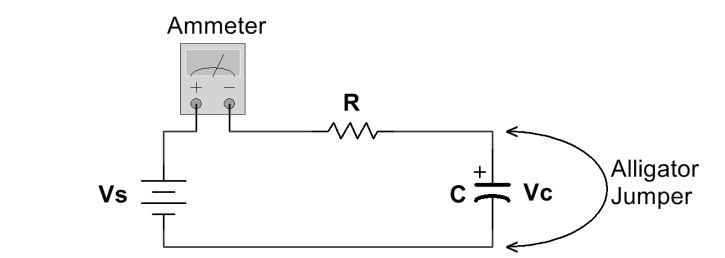
\includegraphics[width = 7 cm]{fig10-1}\\
            \small\textbf{Figure 10-1 Series RC Circuit for Experimental Setup \cite{UNCC-ECE-Dept:2023}}
        \end{center}
    \end{figure} 
    \item Measure the initial current \cite{UNCC-ECE-Dept:2023}.
    \item Calculate the values of $\tau$ and 5$\tau$ in which $\tau$ is equal to $R_{eq}$ times $C_{eq}$ \cite{UNCC-ECE-Dept:2023}.
    \item Collect data by timing the measurements of the current to ever 15 seconds and in order to measure the current remove the alligator clip from the circuit \cite{UNCC-ECE-Dept:2023}.
    \item Take measurements every 15 seconds until 5$\tau$ and possibly further \cite{UNCC-ECE-Dept:2023}.
    \item Repeat the previous 2 steps for trial 2 \cite{UNCC-ECE-Dept:2023}.
    \item Take the average values of the two trials at each measured time \cite{UNCC-ECE-Dept:2023}.
    \item Use the average current to calculate the voltage across the resistor \cite{UNCC-ECE-Dept:2023}.
    \item Solve the voltage across the capacitor, $V_{c}$, which can be solved fro with the voltage accross the resistor $V_{c}$ = ($V_{s}$ - $V_{R}$) \cite{UNCC-ECE-Dept:2023}.  
\end{enumerate}


\section{Results}
$\tau$ =  Initial Current =  \\
5$\tau$ =  \\

\begin{center}
    \small\textbf{Table 10-1: Data Table for RC Time Constant \cite{UNCC-ECE-Dept:2023}}\\
    \begin{tabular}{|p{2 cm}|p{2 cm}|p{2 cm}|p {2 cm}|p {2 cm}|p{2 cm}|}
        \hline
        Time (min:sec) & \multicolumn{3}{|c|}{Current (mA)} & Resistor Voltage (V) & Capacitor Voltage (V) \\
        \hline
        & Trial 1 & Trial 2 & Average & & \\
        \hline
        0:00 & & & & & \\
        \hline
        0:15 & & & & & \\
        \hline
        0:30 & & & & & \\
        \hline
        0:45 & & & & & \\
        \hline
        1:00 & & & & & \\
        \hline
        1:15 & & & & & \\
        \hline
        1:30 & & & & & \\
        \hline
        1:45 & & & & & \\
        \hline
        2:00 & & & & & \\
        \hline
        2:15 & & & & & \\
        \hline
        2:30 & & & & & \\
        \hline
        2:45 & & & & & \\
        \hline
        3:00 & & & & & \\
        \hline
        3:15 & & & & & \\
        \hline
        3:30 & & & & & \\
        \hline
        3:45 & & & & & \\
        \hline
        4:00 & & & & & \\
        \hline
        4:15 & & & & & \\
        \hline
        4:30 & & & & & \\
        \hline
        4:45 & & & & & \\
        \hline
        5:00 & & & & & \\
        \hline
        5:15 & & & & & \\
        \hline
        5:30 & & & & & \\
        \hline
        5:45 & & & & & \\
        \hline
        6:00 & & & & & \\
        \hline
    \end{tabular}
\end{center}



\section{Conclusion}



\bibliography{references}
\bibliographystyle{plain}



\end{document}